%\documentclass[draft]{ws-procs11x85}
%\documentclass[square]{ws-procs11x85}
\documentclass{ws-procs11x85}

\begin{document}

\title{Paper Title}

\author{A. B. AUTHOR$^*$ and C. D. AUTHOR}

\address{University Department, University Name,\\
City, State ZIP/Zone, Country\\
$^*$E-mail: ab\_author@university.com\\
www.university\_name.edu}

\author{A. N. AUTHOR}
 
\address{Group, Laboratory, Street,\\
City, State ZIP/Zone, Country\\
E-mail: an\_author@laboratory.com}

\begin{abstract}
Here should come the abstract.
\end{abstract}

\keywords{keyword 1; keyword 2; keyword 3;}

\bodymatter

\section{Introduction} 

Analysis of protein-protein interactions has a growing potential of
providing a better understanding about collective protein function and cellular machinery.
Such interactions can be modeled as a protein interaction network; that is a
weighted graph where each node represents a protein and each edge represents an
interaction between a pair of proteins, with a weight representing the level of
confidence that this interaction truly exists. Such a structure allows easier
extraction of hidden information due to the analogy with well-known graph
problems.

An important aspect of the analysis of protein interaction networks
is detecting signaling pathways. A signaling pathway is a series of proteins in
which each protein signals its successor to transmit some biological
information through their interaction. Signaling pathways can be viewed as
simple paths in protein interaction networks\cite{kelley}. 

Given a confidence value for each interaction, we can assign an overall
confidence value for the existence of a pathway simply by multiplying the
confidence values of its constituting interactions. An optimal pathway is one
with the highest confidence value. To work in an additive framework instead of
the multiplicative one, edge weights can be assigned logarithmic values of the
original interaction confidence.

\paragraph{Problem} Consider a set $V$ of nodes denoting proteins, and a
probability value $p(u, v)$ denoting interaction confidence for each $u, v \in
V$. A set of undirected weighted edges $E$ can be obtained by adding an edge for
each pair $(u, v)$ with $p(u, v) > 0$, and assigning it a weight $w(p, v) =
-$log[$p(u, v)$]. Now consider the undirected weighted graph $G = (V, E, w)$
representing the protein interaction network, a set of start nodes $S \subset
V$ and a set of end nodes $T \subset V$. We want to find the minimum-weight
simple path of length $m$, starting at any node $s \in S$ and ending at any
node $t \in T$.

Scott et al.\cite{scott} mentioned that the traveling-salesman problem is
polynomial-time reducible to this problem; therefore it is NP-hard. They presented a method
for detecting pathways using a generic technique devised by Alon et
al.\cite{alon} called \textit{color-coding}. The basic idea of this method is to randomly
assign each node in the graph one of $m$ different colors, and search for an
optimal pathway in the restricted domain of colorful pathways. A pathway is
considered colorful if and only if all of its nodes are different in color from
each other. This process is repeated for several iterations until reaching a
given level of confidence that the unknown optimal pathway was among the
colorful ones at some instance. This confidence level builds up with each
iteration by calculating a probability value that an optimal path is indeed
colorful in this iteration. This \textit{success probability} value depends
solely on the pathway length $m$ and doesn�t capitalize on available
information like the network topology and color assignment. As a result, the
method provides a theoretically correct but very conservative success
probability value, and hence loses a very good potential for decreasing the
number of iterations needed to accomplish a given confidence level.

G{\"u}lsoy et al.\cite{gulsoy} presented an enhanced color-coding technique
called \textit{k-hop coloring}. In essence, k-hop coloring makes use of
knowing the network topology and the node colors to assign the network a
maximal value $k$ such that the network is k-hop colorable. A colored network is
k-hop colorable if the shortest path between any pair of same-color nodes is
more than $k$ hops in length. This additional piece of information allows for
higher success probability in each iteration, with a higher $k$ value resulting
in a higher success probability. However, an obvious limitation is that the
subnetworks with higher level of connectivity diminishe the $k$ value assigned
to the whole network. For example, a network containing a clique of size $m$
cannot be colored with ($m-1$)-hop coloring using $m$ colors\cite{gulsoy}.

\paragraph{Contribution} Our motivation comes from the need for a deeper
understanding of the relation between network topology, random color assignment
and success probability. We study the possibility of assigning $k$ values to
nodes on an individual basis instead of a single $k$ value for the whole
network. We also study how this reflects on the resulting success probability
for each iteration. We examine the idea that a pathway whose nodes are assigned
different $k$ values should result in a higher success probability than if we
only consider the minimum of these $k$ values for all nodes. Given different
$k$ values for each node on a pathway, we show how to obtain a better bound on
success probability.



Based on these findings, We present a new method for detecting signaling
pathways in protein interaction networks using an enhanced k-hop coloring
technique. For a required optimal pathway of length $m$, we start by assigning
one of $m$ colors to each node in the graph, then we extract the optimal
colorful pathway. We then calculate our new bound on success probability. We
repeat this process until the cumulative success probability is at least equal
to a given confidence level. Although our theoretical findings are based on
assuming the knowledge of the $k$ values assigned to the unknown global optimal
pathway, we empirically show that the local optimal pathway extracted from the
domain of colorful pathways actually fits the purpose.

We provide validation experiments to test the biological significance of our
results. We use \textit{weight p-value} and \textit{functional enrichment} as
validation measures. We also compare the performance of our method against the
one presented by Scott et al.\cite{scott} with respect to how fast our method
reaches a given confidence level as opposed to theirs.

The rest of the paper is organized as follows. Section 2 discusses the
background and related work. Section 3 explains how to obtain a tighter bound on
success probability and describes our enhanced k-hop coloring method. Section 4
shows the experiments performed and their results. Section 5 is the conclusion
of the paper.


\section{Background}

Some different but closely related problems have been studied in the literature.
Zhao et al.\cite{zhao} used integer linear programming to find signaling networks
in protein interaction networks. They formulated the problem as a linear
optimization problem of finding maximum weight subnetwork with a given size.
This approach is concerned with finding signaling subnetworks in their general
form rather than linear pathways. Kelley et al.\cite{kelley} detected conserved
signaling pathways between related organisms by performing global alignment
between their protein interaction networks. They scored each pathway in terms
of probability of true homology between aligned pair of proteins, as well as
probability of true interactions between pairs of proteins along the pathway.
This approach detects conserved pathways only and requires coupling between two
datasets. Shlomi et al.\cite{shlomi} introduced QPath, a method for querying
protein interaction networks for pathways using known homologous pathways as
queries. They scored results based on their similarity to the query, number of
insertions and deletions used, as well as the reliability of their interactions.
This method only detects pathways that are similar to a given one.

On the other hand, the problem we address has also been studied in the
literature. Lu et al.\cite{lu} presented a divide-and-conquer algorithm for
finding generic pathway structures in protein interaction networks. They
recursively partitioned the network into two sets of vertices, enumerated
substructures present in each set, and then built larger structures from them.
They assumed that all edges have the same weight and scored the resulting
pathway structures based on the biological function relatedness of their nodes
to the given source and destination nodes. We are more interested in detecting
pathways based on confidence in interactions rather than similarity of
proteins.

Steffen et al.\cite{steffen} studied detecting signaling pathways in protein
interaction networks as guided by expression data. They listed all pathway
candidates in a protein interaction network using exhaustive search. They
scored each candidate based on how similar the expression profiles of its
genes are. Bebek et al.\cite{bebek} presented a method called PathFinder for
finding new signaling pathways using association rules of known ones. They
started with mining association rules for known pathways, guided by the
knowledge of functional annotations of their proteins. They then performed an
exhaustive search for candidate pathways. From these candidates, they selected
the ones having at least a certain number of the known association rules and an
average interaction weight above a given threshold. The drawback of both of
these methods is that the time complexity of exhaustive graph search is
exponential in terms of the network size, and hence is very inefficient.

Gitter et al.\cite{gitter} presented a method for discovering signaling
pathways by adding edge orientation to protein interaction networks. They
selected an optimal orientation of all edges in the network that maximizes the
weights of all satisfied length-bound paths. A path is satisfied if it follows
the same direction along its edges from a source node to a destination node.
They proved that this problem is NP-hard. They provided two approximation
algorithms for it based on available solution methods for weighted Boolean
satisfiability, and a third algorithm based on probabilistic selection. As
shown in their results, these methods do not scale well with increasing the
number of source and destination nodes and the required path length.

The present work builds on the method presented by Scott et al.\cite{scott} for
detecting signaling pathways in protein interaction networks using color coding.
It also enhances the model presented by G{\"u}lsoy et al.\cite{gulsoy} for
topology-aware color coding. We indroduced both methods in section 1.

\section{Methods}

In this section, we start by properly formulating the problem and defining
common terms that we use in our methods. We then present new thoughts about
pathway detection using color coding. We study the opportunity of more involving
of network topology in our calculation to obtain a better success probability,
and hence needing less number of iterations and improving performance. Last, we
present an enhanced color-coding method for detecting pathways in protein
interaction networks.

\subsection{Problem Formulation and Term Definition}
Given a graph $G = (V, E, w)$, where $V$ is its set of nodes, $E$ is its set of
edges and $w$ is the edge-weight function, and given a set $S \subset V$ and a
path length $m$. Assume $P(i)$ is the set of all simple paths of length $m$
starting at any node $s \in S$ and ending at node $i$. Our goal is to find, for
each node $i$, the path $p \in P(i)$ whose sum of edge weights is minimum.

The following are the definition of some commonly used terms:
\begin{arabiclist}[3]
\item {\scshape k neighborhood}: for a given node $v \in V$ and an integer $k$,
the $k$ neighborhood of $v$ is a set of nodes  $U \subset V$ where a node $u \in
U$ if and only if $u$ can be reached from $v$ in $k$ hops or less.
\item {\scshape max\_k}: for a given node $v \in V$, $max\_k(v)$ is the maximal
value of $k$ such that $\forall u \in k$ neighborhood of $v$, the color assigned
to $u$ is not equal to the color assigned to $v$.
\item {\scshape max\_k configuration}: for a given path $P$, the $max\_k$
configuration of $P$ is the sequence of $max\_k$ values corresponding to the
sequence of nodes in $P$.
\end{arabiclist}

\subsection{Success Probability: a Tighter Bound}

Based on the work presented by Scott et al.\cite{scott}, a generic color-coding
approach to solving the problem consists of three main steps. The first step is
coloring the network; $\forall v \in V$ we independently select a color drawn
uniformly at random from a set of $m$ different colors. The second step is
finding an optimal colorful path; $\forall v \in V$ we want to find the
minimum-weight colorful path of length $m$ starting in $S$ and ending at $v$,
and then we extract the minimum of these paths. The third step is calculating
the success probability $P_s$; we calculate a lower bound on the probability
that the unknown overall optimal path is indeed colorful, hence the probability
that it is indeed the optimal colorful one we found. These three steps are
repeated $r$ times until $1 - \prod_{i=1}^r [1 - P_s(i)] \geq \epsilon$, where
$\epsilon$ is a required confidence level. It is obvious that a higher success
probability would result in less number of iterations required, hence less
execution time.

Calculating success probability in general is a counting problem. The
generic rule is:
\begin{equation}
P_s = \frac{m!}{N_c}
\label{eq1}
\end{equation} 
where $m!$ is the number of coloring possibilities in which the path is
colorful, and $N_c$ denotes the total number of coloring possibilities for the
path. Scott et al.\cite{scott} calculated $N_c$ as equal to $m^m$. This
calculation considered no restrictions on the color selection of each node, and
discarded available knowledge of the network topology and colors already
assigned to its nodes.

As guided by G{\"u}lsoy et al.\cite{gulsoy}, knowing the network topology can be
useful in calculating success probability, specifically the number of coloring
possibilities of the optimal path. $\forall v \in V$, $\forall u \in k$
neighborhood of $v$, if the color of $u$ is not equal to that of $v$, then the
number of coloring possibilities can be calculated as follows:
\begin{equation}
N_c \leq (m - k)^{m - k} \prod_{i=0}^{k-1} (m - i)  \leq  m^m
\end{equation}
which, according to equation (\ref{eq1}), results in a lower bound on success
probability that is higher in value if $k > 0$. However, according to this
scheme, the node with a minimum value of $max\_k$ dominates the whole network,
which produces a correct but very conservative lower bound on success
probability.

Our approach relies on individual $max\_k$ values of all nodes in an optimal
path. Assuming knowledge of the $max\_k$ configuration of the optimal path, we
use it to calculate $N_c$ under the restrictions induced by these values. We
also assume that each node in the path is not connected to any other nodes
except the ones before and after it in the path. This assumption is valid
because any more connections will only induce more coloring restrictions,
causing $N_c$ to decrease; therefore we get a solid upper bound on $N_c$, hence
a solid lower bound on $P_s$ according to equation (\ref{eq1}). For a given node
$v$ in a given path, all $max\_k(v)$ nodes in either direction from $v$ are not allowed to have the same
color as $v$. We represent this rule as an unweighted constraint graph $W = (H,
L)$ where $H$ is its set of nodes and $L$ is its set of edges. $H$ contains a
node corresponding to each node in the path, and $L$ contains an edge for each
pair of nodes that are not allowed to have the same color, according to the
aforementioned rule. Figure \ref{maxk} shows an example of a path, its $max\_k$
configuration and the corresponding constraint graph $W$. The problem now
translates to calculating the value of the chromatic polynomial $P(W, m)$: the
number of ways of coloring $W$ using $m$ colors without any pair of adjacent
nodes having the same color. We calculate this value using the following
edge-contraction recursive rule based on the fundamental reduction
theorem\cite{dong}:
\begin{equation}
P(W, m) = P(W - uv, m) - P(W / uv, m)
\end{equation}
where $u$ and $v$ are any pair of adjacent nodes, $W - uv$ is the graph $W$
after removing the edge $uv$, and $W / uv$ is the graph $W$ after merging the
nodes $u$ and $v$.

\begin{figure}[h]
\centerline{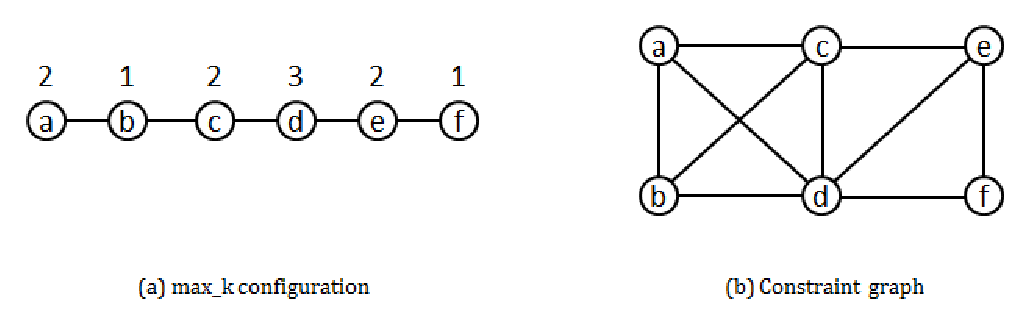
\psfig{file=maxk.eps,width=16.5cm}}
\caption{(a) An example 6-node path with its $max\_k$ configuration shown above
it. Each $max\_k$ value translates to the number of nodes that have to be of
different color on either direction. (b) The corresponding constraint graph $W$:
each pair of adjacent nodes have to be of different color. Finding the value of
the chromatic polynomial $P(W, m)$ yields the number of coloring possibilities
for the path under the given constraints.}
\label{maxk}
\end{figure}

According to this method, the value of $N_c$ for the example path shown in
Figure \ref{maxk}(a) is 5,760, while Scott et al.\cite{scott} and G{\"u}lsoy et
al.\cite{gulsoy} would respectively yield $N_c$ = 46,656 and 18,750 for the same
example. Such a decrease in the value of $N_c$ leads to an increase in the value
of $P_s$ according to equation (\ref{eq1}).

\subsection{Method: Enhanced k-hop Coloring}
Here we detail our method. We start by asserting that we have no knowledge about
the optimal path, but we use the local optimal as a replacement and
experimentally test the correctness of this approach. Then we explain the
algorithm in detail.

\section{Experiments}

\subsection{Datasets}
Here we list the datasets used in experiments. I think we can use the MINT
datasets for multiple organisms.

\subsection{Validation Experiments}
Here we list the validation experiments we did and their results. I think we
should do some validation experiments similar to those done in Sharan's paper,
using weight p-value and functional enrichment as validitiy measures.

\subsubsection{Validation using Weight p-value}
For each dataset we use, we should obtain the 99 percent confidence optimal
pathway and compare it with optimal pathways obtained we obtain from random
networks. We generate random networks by shuffling edges of the original
network. The weight p-value is the percentage of cases where the algorithm
produces a more optimal pathway when run on one of these random networks.

\subsubsection{Validation using Functional Enrichment}
 For each dataset, we we obtain the 99 percent confidence optimal pathway and
 test its functional enrichment. For each GO term appearing on the dataset
 proteins, we count the total number of proteins annotated by it and the
 number of proteins in the resulting pathway annotated by it. We use these
 numbers, along with the total number of proteins and the number of proteins in
 the pathway, as parameters for a hypergeometric test (I still have to develop
 further understanding about the details of this test). The maximum enrichment
 value for any of the tested GO terms gives us the final functional enrichment
 p-value.

\subsection{Comparison with Sharan}
This is just a temporary title for this subsection, I'm not very sure what to
name it.

\paragraph{}
We measure the time and number of iterations needed by our method to obtain
70\%, 90\% and 99\% confidence pathways of lengths 6, 7, 8 and 9 nodes. We
compare these numbers against the ones by Sharan's method for the same cases.

\paragraph{}
We run our method for 500 iterations and measure the incremental success
probabilty against iteration number. We do this experiment many times take the
average curve. We do the same experiment using Sharan's method and obtain a
second curve. We also measure the average practical success probability, which
is the observed probability that the DP algorithm finds the optimal solution in
a certain iteration or before it. We compare the three curves targetting two
conclusions: (1) our method is experimentally solid because our calculated
success probabiilities are lower than the observed ones; and (2) our method
outperforms Sharan's method.

\section{Conclusion}
Here goes the conclusion.


\bibliographystyle{ws-procs11x85}
\bibliography{references}

\end{document}
